\section{模拟求解}

\subsection{算法描述}

蒙特卡罗方法(Monte Carlo method),也称统计模拟方法,与它对于的是确定性算法。其基本思想,通过某种“实验”的方法,以这种事件出现的频率估计这一随机事件的概率,或者得到这个随机变量的某些数字特征。

\begin{itemize}
\item \textbf{蒙特卡罗方法}:采样越多,越近似最优解;
\item \textbf{拉斯维加斯方法}:采样越多,越有机会找到最优解。
\end{itemize}

\subsection{代码及结果}

我们用蒙特卡罗算法立即可以写出下面简单的程序:

大概思路是:给出策略和实验次数,进行模拟,每次试验,变量 \verb|car| 和 \verb|first_choice| 分别取随机数初始化车的门和第一次选择的门。如果策略为坚持 \verb|stick|,第一次选择的门为车的门,则赢得汽车次数 \verb|winnings| 进行加一,否则不变;如果策略为改变 \verb|change|,第一次选择的门不为车的门,则赢得汽车次数加一,否则不变。

\lstinputlisting[language=Matlab]{code/Monte_Carlo.m}

得到如下输出

\begin{figure}[H]
	\centering
	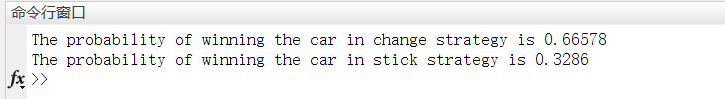
\includegraphics[width=12cm]{figure/out1.png}
\end{figure}

上面这个程序过于简陋了,于是我们利用矩阵重写一个并添加可视化绘图代码如下:

\lstinputlisting[language=Matlab]{code/m_hall.m}

得到如下输出

\begin{figure}[htbp]
	\centering
	\begin{minipage}[t]{0.48\textwidth}
		\centering
		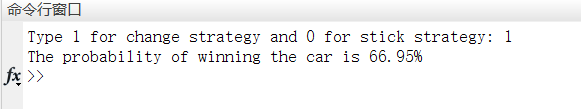
\includegraphics[width=8cm]{figure/out2(1).png}
	\end{minipage}
	\begin{minipage}[t]{0.48\textwidth}
		\centering
		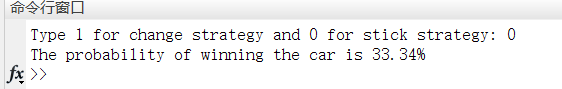
\includegraphics[width=8cm]{figure/out2(2).png}
	\end{minipage}
\end{figure}

绘图结果为:

\begin{figure}[htbp]
	\centering
	\begin{minipage}[t]{0.48\textwidth}
		\centering
		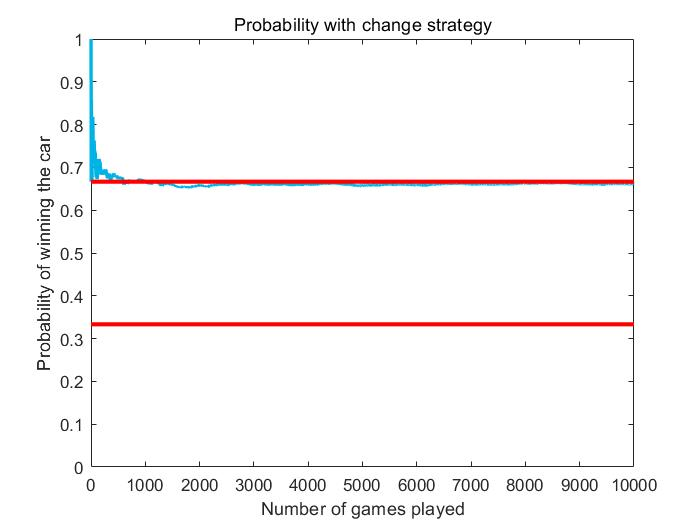
\includegraphics[width=8cm]{figure/change.jpg}
		\caption{Probability with change strategy}
	\end{minipage}
	\begin{minipage}[t]{0.48\textwidth}
		\centering
		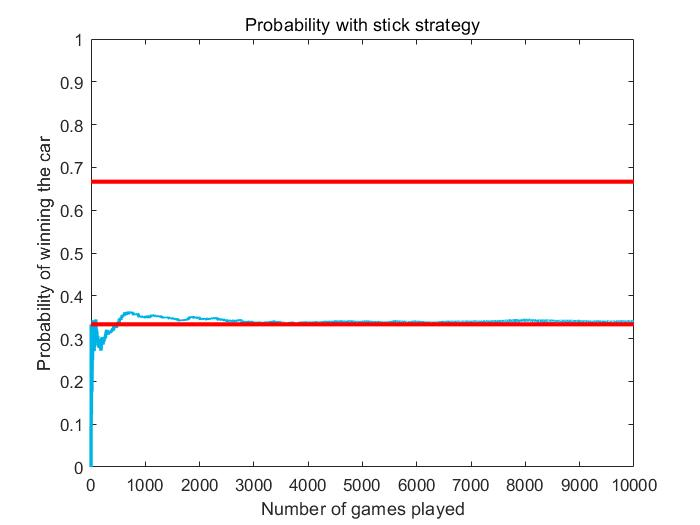
\includegraphics[width=8cm]{figure/stick.jpg}
		\caption{Probability with stick strategy}
	\end{minipage}
\end{figure}